% Options for packages loaded elsewhere
\PassOptionsToPackage{unicode}{hyperref}
\PassOptionsToPackage{hyphens}{url}
%
\documentclass[
]{book}
\usepackage{amsmath,amssymb}
\usepackage{lmodern}
\usepackage{iftex}
\ifPDFTeX
  \usepackage[T1]{fontenc}
  \usepackage[utf8]{inputenc}
  \usepackage{textcomp} % provide euro and other symbols
\else % if luatex or xetex
  \usepackage{unicode-math}
  \defaultfontfeatures{Scale=MatchLowercase}
  \defaultfontfeatures[\rmfamily]{Ligatures=TeX,Scale=1}
\fi
% Use upquote if available, for straight quotes in verbatim environments
\IfFileExists{upquote.sty}{\usepackage{upquote}}{}
\IfFileExists{microtype.sty}{% use microtype if available
  \usepackage[]{microtype}
  \UseMicrotypeSet[protrusion]{basicmath} % disable protrusion for tt fonts
}{}
\makeatletter
\@ifundefined{KOMAClassName}{% if non-KOMA class
  \IfFileExists{parskip.sty}{%
    \usepackage{parskip}
  }{% else
    \setlength{\parindent}{0pt}
    \setlength{\parskip}{6pt plus 2pt minus 1pt}}
}{% if KOMA class
  \KOMAoptions{parskip=half}}
\makeatother
\usepackage{xcolor}
\IfFileExists{xurl.sty}{\usepackage{xurl}}{} % add URL line breaks if available
\IfFileExists{bookmark.sty}{\usepackage{bookmark}}{\usepackage{hyperref}}
\hypersetup{
  pdftitle={Dominica's Preparedness ~Diagnosis},
  pdfauthor={CARICOM},
  hidelinks,
  pdfcreator={LaTeX via pandoc}}
\urlstyle{same} % disable monospaced font for URLs
\usepackage{color}
\usepackage{fancyvrb}
\newcommand{\VerbBar}{|}
\newcommand{\VERB}{\Verb[commandchars=\\\{\}]}
\DefineVerbatimEnvironment{Highlighting}{Verbatim}{commandchars=\\\{\}}
% Add ',fontsize=\small' for more characters per line
\usepackage{framed}
\definecolor{shadecolor}{RGB}{248,248,248}
\newenvironment{Shaded}{\begin{snugshade}}{\end{snugshade}}
\newcommand{\AlertTok}[1]{\textcolor[rgb]{0.94,0.16,0.16}{#1}}
\newcommand{\AnnotationTok}[1]{\textcolor[rgb]{0.56,0.35,0.01}{\textbf{\textit{#1}}}}
\newcommand{\AttributeTok}[1]{\textcolor[rgb]{0.77,0.63,0.00}{#1}}
\newcommand{\BaseNTok}[1]{\textcolor[rgb]{0.00,0.00,0.81}{#1}}
\newcommand{\BuiltInTok}[1]{#1}
\newcommand{\CharTok}[1]{\textcolor[rgb]{0.31,0.60,0.02}{#1}}
\newcommand{\CommentTok}[1]{\textcolor[rgb]{0.56,0.35,0.01}{\textit{#1}}}
\newcommand{\CommentVarTok}[1]{\textcolor[rgb]{0.56,0.35,0.01}{\textbf{\textit{#1}}}}
\newcommand{\ConstantTok}[1]{\textcolor[rgb]{0.00,0.00,0.00}{#1}}
\newcommand{\ControlFlowTok}[1]{\textcolor[rgb]{0.13,0.29,0.53}{\textbf{#1}}}
\newcommand{\DataTypeTok}[1]{\textcolor[rgb]{0.13,0.29,0.53}{#1}}
\newcommand{\DecValTok}[1]{\textcolor[rgb]{0.00,0.00,0.81}{#1}}
\newcommand{\DocumentationTok}[1]{\textcolor[rgb]{0.56,0.35,0.01}{\textbf{\textit{#1}}}}
\newcommand{\ErrorTok}[1]{\textcolor[rgb]{0.64,0.00,0.00}{\textbf{#1}}}
\newcommand{\ExtensionTok}[1]{#1}
\newcommand{\FloatTok}[1]{\textcolor[rgb]{0.00,0.00,0.81}{#1}}
\newcommand{\FunctionTok}[1]{\textcolor[rgb]{0.00,0.00,0.00}{#1}}
\newcommand{\ImportTok}[1]{#1}
\newcommand{\InformationTok}[1]{\textcolor[rgb]{0.56,0.35,0.01}{\textbf{\textit{#1}}}}
\newcommand{\KeywordTok}[1]{\textcolor[rgb]{0.13,0.29,0.53}{\textbf{#1}}}
\newcommand{\NormalTok}[1]{#1}
\newcommand{\OperatorTok}[1]{\textcolor[rgb]{0.81,0.36,0.00}{\textbf{#1}}}
\newcommand{\OtherTok}[1]{\textcolor[rgb]{0.56,0.35,0.01}{#1}}
\newcommand{\PreprocessorTok}[1]{\textcolor[rgb]{0.56,0.35,0.01}{\textit{#1}}}
\newcommand{\RegionMarkerTok}[1]{#1}
\newcommand{\SpecialCharTok}[1]{\textcolor[rgb]{0.00,0.00,0.00}{#1}}
\newcommand{\SpecialStringTok}[1]{\textcolor[rgb]{0.31,0.60,0.02}{#1}}
\newcommand{\StringTok}[1]{\textcolor[rgb]{0.31,0.60,0.02}{#1}}
\newcommand{\VariableTok}[1]{\textcolor[rgb]{0.00,0.00,0.00}{#1}}
\newcommand{\VerbatimStringTok}[1]{\textcolor[rgb]{0.31,0.60,0.02}{#1}}
\newcommand{\WarningTok}[1]{\textcolor[rgb]{0.56,0.35,0.01}{\textbf{\textit{#1}}}}
\usepackage{longtable,booktabs,array}
\usepackage{calc} % for calculating minipage widths
% Correct order of tables after \paragraph or \subparagraph
\usepackage{etoolbox}
\makeatletter
\patchcmd\longtable{\par}{\if@noskipsec\mbox{}\fi\par}{}{}
\makeatother
% Allow footnotes in longtable head/foot
\IfFileExists{footnotehyper.sty}{\usepackage{footnotehyper}}{\usepackage{footnote}}
\makesavenoteenv{longtable}
\usepackage{graphicx}
\makeatletter
\def\maxwidth{\ifdim\Gin@nat@width>\linewidth\linewidth\else\Gin@nat@width\fi}
\def\maxheight{\ifdim\Gin@nat@height>\textheight\textheight\else\Gin@nat@height\fi}
\makeatother
% Scale images if necessary, so that they will not overflow the page
% margins by default, and it is still possible to overwrite the defaults
% using explicit options in \includegraphics[width, height, ...]{}
\setkeys{Gin}{width=\maxwidth,height=\maxheight,keepaspectratio}
% Set default figure placement to htbp
\makeatletter
\def\fps@figure{htbp}
\makeatother
\setlength{\emergencystretch}{3em} % prevent overfull lines
\providecommand{\tightlist}{%
  \setlength{\itemsep}{0pt}\setlength{\parskip}{0pt}}
\setcounter{secnumdepth}{5}
\usepackage{booktabs}
\ifLuaTeX
  \usepackage{selnolig}  % disable illegal ligatures
\fi
\usepackage[]{natbib}
\bibliographystyle{apalike}

\title{Dominica's Preparedness ~Diagnosis}
\author{CARICOM}
\date{2022-05-28}

\begin{document}
\maketitle

{
\setcounter{tocdepth}{1}
\tableofcontents
}
\hypertarget{welcome}{%
\chapter*{Welcome}\label{welcome}}
\addcontentsline{toc}{chapter}{Welcome}

This is the website for Dominica's Preparedness Diagnosis by CARICOM and CLEAR LAC!

\hypertarget{part-preface}{%
\part{Preface}\label{part-preface}}

\hypertarget{acknowledgements}{%
\chapter*{Acknowledgements}\label{acknowledgements}}
\addcontentsline{toc}{chapter}{Acknowledgements}

The CLEAR LAC team wishes to thank everyone involved in preparing this document. Especially to:

\begin{itemize}
\item
  Dr.~Kyra Paul, Dominica´s Executive Coordinator for the Collaboration on RBM.
\item
  Mrs.~Leah St.~Jean, Dominica's Junior Executive Coordinator for the Collaboration on RBM.
\item
  Mrs.~Maurya West-Myers and Mr.~Leonardo Lemes from the Global Evaluation Initiative
\item
  Mrs.~Hipolina Joseph and Ms.~Stacy-Ann Barnes, from the CARICOM Secretariat
\item
  The team of the CLEAR LAC´s interns who supported in the process of preparing this diagnosis: Alexia Galarza, Carolina Zepeda, Gisela Hurtado, Mariana Espinoza, Emilio Olmos and Lothar Rojas.
\end{itemize}

\hypertarget{acronyms-and-abbreviations}{%
\chapter*{Acronyms and abbreviations}\label{acronyms-and-abbreviations}}
\addcontentsline{toc}{chapter}{Acronyms and abbreviations}

\textbf{CARICOM} -The Caribbean Community

\textbf{CLEAR LAC} - Center for Learning on Evaluation and Results for Latin America and Caribbean

\textbf{CREAD} - Climate Resilience Executive Agency of Dominica

\textbf{CRRP} -- Climate Resilience and Recovery Plan 2020 -- 2030

\textbf{NRDS} -- National Resilience Development Strategy 2030

\textbf{PSIP} -- Public Sector Investment Programme

\hypertarget{list-of-figures-and-tables}{%
\chapter*{List of figures and tables}\label{list-of-figures-and-tables}}
\addcontentsline{toc}{chapter}{List of figures and tables}

\textbf{Figure 1.} Theory of Change

\textbf{Figure 2.} Dimensions of an ideal RBM system

\textbf{Figure 3.} Working Process defined for the CARICOM Collaboration

\textbf{Figure 4.} Stages of the Preparedness Diagnostic

\textbf{Figure 5.} Level of progress of the Ideal RBM System

\textbf{Figure 6.} From an ideal RBM system to the roadmaps

\textbf{Figure 7.} Learning loop

\textbf{Figure 8.} How to identify the current level of the RBM system maturity

\textbf{Table 1.} Dominica's Preparedness Diagnostic Numbers

\textbf{Table 2.} General Statistics of Dominica

\textbf{Table 3.} Stakeholders Analysis

\textbf{Table 4:} Elements and sub-elements of the Ideal RBM System

\textbf{Table 5:} Detailed results of the Preparedness Diagnostic for Dominica

\textbf{Table 6.} List of participants in the Preparedness Diagnostic

\hypertarget{definitions-and-concepts}{%
\chapter*{Definitions and concepts}\label{definitions-and-concepts}}
\addcontentsline{toc}{chapter}{Definitions and concepts}

\textbf{Evaluation} - The systematic and objective assessment of an ongoing or completed project, programme, or policy, including its design, implementation, and results.

\textbf{Monitoring} -- The continuous and systematic collection of data on specified indicators, to provide information on the extent to which resources have been used and what outputs have been achieved or produced.

\textbf{Result} - Clearly defined and demonstrable output, outcome, or impact (intended or unintended, positive and/or negative) of an intervention.

\textbf{Results-Based Management System (RBM System)}\footnote{This concept was developed following internationally recognised standards and approaches and contextualised to the particular case of CARICOM} - It is a global and systemic approach to management that orients all strategies, actions, and resources (both human and material) towards improving decision-making and the achievement and measurement of clearly defined and demonstrable results expected by governments and institutions, whether national, regional, or global.

This systemic approach can be analysed at three levels (considering all the relationships that may exist between them) for CARICOM: the national level, the regional institutions level, and the whole-regional / CARICOM level. These levels are individual and do not have a defined hierarchy, as they have their own institutional, human, financial and multidimensional contextual characteristics that make them independent of each other. Nevertheless, the articulation between them is relevant to understanding how RBM operates in the region.

The RBM system can, in turn, be composed of different sub-systems (that are systems by themselves). Some of the most important, but not the only ones, are: the monitoring and evaluation (M\&E) sub-system (with the formal document that institutionalises it: the M\&E Policy or Framework, if it exists); the data and information sub-system, which generates, processes, systematises and publishes relevant information to know and scale the multidimensional situation of the country or institution and thus identify problems to be addressed and guide decision-making; the human resources management sub-system, which builds and constantly strengthens the necessary capacities to have the staff with the capabilities to carry out the M\&E and RBM activities necessary to achieve and measure the expected results, etc.

RBM policies, on the other hand, are key elements of a sustainable RBM system but are not, by themselves, the system. RBM policies are the normative framework that: defines how the RBM system will be structured; establishes the guiding principles for the results-oriented approach; communicates what RBM entails for the country, institution or region; identifies stakeholders to be involved and their responsibilities; and identifies the needs to execute the necessary activities, among other elements. National, institutional, and regional RBM systems linkages may be established in RBM policies, which may have shared elements.

In this way, we should not confuse the RBM system with technological applications, platforms, software, or digital repositories with data or information contained and systematised, with the other sub-systems (described above) that conforms it, or with the RBM policies; but we should assume that to have a fully operational RBM system, it is necessary to seek a good articulation between all the sub-systems and levels, so we can achieve and measure the expected results, both at the national and regional levels.

\hypertarget{part-preparedness-diagnosis}{%
\part{Preparedness Diagnosis}\label{part-preparedness-diagnosis}}

\hypertarget{introduction}{%
\chapter{Introduction}\label{introduction}}

In July 2014, the Conference of Heads of Government of the Caribbean Community (CARICOM), approved the CARICOM Strategic Plan 2015-2019 which articulated the need for a more results-focused approach to programme and project management, and committed the Caribbean Community Secretariat to establish a planning, monitoring and evaluation (M\&E), and reporting system based on the principles of Results-Based Management (RBM). In executing the tenets of the Community Strategic Plan, all implementing partners have expressed concern about an \emph{implementation deficit}. This has resulted in poor implementation of public policy and Regional Public Goods in many Member States, culminating in low rates of successful program and project implementation across the Community.

Efforts to address the \emph{implementation deficit}, to promote a more results-focused approach to programme and project management, and to strengthen RBM in the Community commenced in 2016 with the engagement of the consulting firm Baastel, to develop the CARICOM RBM System and support its institutionalisation at the CARICOM Secretariat. In October 2019, the CARICOM Secretariat requested technical assistance\footnote{With non-lending Technical Assistance (TA) the Bank helps clients to implement reform and/or strengthen institutions. Qualified TA activity must meet the following criteria: have a primary intent of enabling an external client to implement reform and/or strengthen institutions; be linked to a Bank unit with clear accountability for the service provided.} from the World Bank's Independent Evaluation Group (IEG) to continue these efforts by supporting CARICOM in strengthening a result-oriented culture across the Community, which includes three implementing partners, the Member States, Regional Institutions, and the CARICOM Secretariat.

As part of the collaboration, the IEG and CLEAR LAC under the Global Evaluation Initiative (GEI) agreed to provide technical assistance in the establishment and institutionalisation of RBM policies, in addition to the Secretariat, to three pilot Member States (Dominica, Jamaica, and Saint Lucia) and three pilot Regional Institutions (the Caribbean Development Fund, the Caribbean Examinations Council, and the CARICOM Implementation Agency for Crime and Security). These pilots will serve as champions to support capacity strengthening in the remaining Member States and Regional Institutions, in collaboration with IEG and the CARICOM Secretariat.

In order to establish a customize roadmap to strengthen the pilot´s RBM Systems, a Preparedness Diagnostic was identified as a first step of the collaboration to assess the level of maturity of the systems and identify specific contextual and organizational features and milestones to be achieved over a period of five years.
This report presents the findings from the Preparedness Diagnostic for the Commonwealth of Dominica (Dominica from here on). The report provides information on the existing strengthens and opportunities to develop a sustainable RBM System in the Member State.

The report consists of six sections, aside of the introduction. \protect\hyperlink{section2}{Section 2} will present Dominica's position on the results of the Preparedness Diagnostic. \protect\hyperlink{section3}{Section 3} presents the methodology description which includes the Theory of Change of this activity; the Preparedness Diagnostic stages, and the ``Ideal RBM System,'' which consists of a four dimension benchmark for the assessment.

\protect\hyperlink{section4}{Section 4} contains general and contextual information of Dominica. This section also addresses the interest, expectations and challenges that may arise through the implementation of an RBM system with a whole of government approach. Additionally, progress on the development of their RBM system based on the four dimensions mentioned is presented under this section.
\protect\hyperlink{section5}{Section 5} presents the main findings and level of progress for Dominica in each of the four dimensions. Finally, \protect\hyperlink{section6}{Section 6} introduces the process for building a contextualized roadmap for advancing towards a sustainable RBM system for Dominica, as well as a stakeholders' contribution analysis.

After reading this report, the reader will obtain a clear idea of the existing practices and elements to strength on and advance towards achieving a sustainable RBM system based on key elements. The report may also be used to guide discussions among relevant stakeholders to support sensitisation of key stakeholders in the area of RBM practices; to share best practices with other Member States; as well as to promote existing promising practices that are being implemented.
Specifically, within the framework of this collaboration, the report represents the main input for the development of the contextualized medium-term roadmaps which will be facilitated through participatory workshops and engagements.

\hypertarget{section2}{%
\chapter{Dominica's position on the Preparedness Diagnostic}\label{section2}}

Cross-references make it easier for your readers to find and link to elements in your book.

\hypertarget{chapters-and-sub-chapters}{%
\section{Chapters and sub-chapters}\label{chapters-and-sub-chapters}}

There are two steps to cross-reference any heading:

\begin{enumerate}
\def\labelenumi{\arabic{enumi}.}
\tightlist
\item
  Label the heading: \texttt{\#\ Hello\ world\ \{\#nice-label\}}.

  \begin{itemize}
  \tightlist
  \item
    Leave the label off if you like the automated heading generated based on your heading title: for example, \texttt{\#\ Hello\ world} = \texttt{\#\ Hello\ world\ \{\#hello-world\}}.
  \item
    To label an un-numbered heading, use: \texttt{\#\ Hello\ world\ \{-\#nice-label\}} or \texttt{\{\#\ Hello\ world\ .unnumbered\}}.
  \end{itemize}
\item
  Next, reference the labeled heading anywhere in the text using \texttt{\textbackslash{}@ref(nice-label)}; for example, please see Chapter \ref{cross}.

  \begin{itemize}
  \tightlist
  \item
    If you prefer text as the link instead of a numbered reference use: \protect\hyperlink{cross}{any text you want can go here}.
  \end{itemize}
\end{enumerate}

\hypertarget{captioned-figures-and-tables}{%
\section{Captioned figures and tables}\label{captioned-figures-and-tables}}

Figures and tables \emph{with captions} can also be cross-referenced from elsewhere in your book using \texttt{\textbackslash{}@ref(fig:chunk-label)} and \texttt{\textbackslash{}@ref(tab:chunk-label)}, respectively.

See Figure \ref{fig:nice-fig}.

\begin{Shaded}
\begin{Highlighting}[]
\FunctionTok{par}\NormalTok{(}\AttributeTok{mar =} \FunctionTok{c}\NormalTok{(}\DecValTok{4}\NormalTok{, }\DecValTok{4}\NormalTok{, .}\DecValTok{1}\NormalTok{, .}\DecValTok{1}\NormalTok{))}
\FunctionTok{plot}\NormalTok{(pressure, }\AttributeTok{type =} \StringTok{\textquotesingle{}b\textquotesingle{}}\NormalTok{, }\AttributeTok{pch =} \DecValTok{19}\NormalTok{)}
\end{Highlighting}
\end{Shaded}

\begin{figure}

{\centering 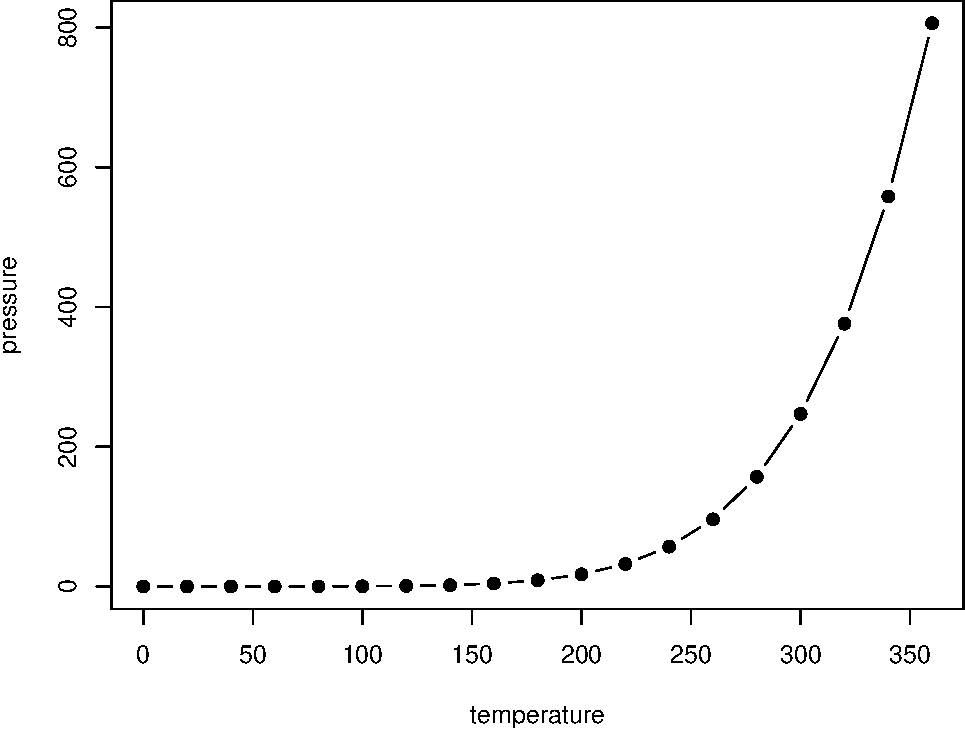
\includegraphics[width=0.8\linewidth]{06-section2_files/figure-latex/nice-fig-1} 

}

\caption{Here is a nice figure!}\label{fig:nice-fig}
\end{figure}

Don't miss Table \ref{tab:nice-tab}.

\begin{Shaded}
\begin{Highlighting}[]
\NormalTok{knitr}\SpecialCharTok{::}\FunctionTok{kable}\NormalTok{(}
  \FunctionTok{head}\NormalTok{(pressure, }\DecValTok{10}\NormalTok{), }\AttributeTok{caption =} \StringTok{\textquotesingle{}Here is a nice table!\textquotesingle{}}\NormalTok{,}
  \AttributeTok{booktabs =} \ConstantTok{TRUE}
\NormalTok{)}
\end{Highlighting}
\end{Shaded}

\begin{table}

\caption{\label{tab:nice-tab}Here is a nice table!}
\centering
\begin{tabular}[t]{rr}
\toprule
temperature & pressure\\
\midrule
0 & 0.0002\\
20 & 0.0012\\
40 & 0.0060\\
60 & 0.0300\\
80 & 0.0900\\
\addlinespace
100 & 0.2700\\
120 & 0.7500\\
140 & 1.8500\\
160 & 4.2000\\
180 & 8.8000\\
\bottomrule
\end{tabular}
\end{table}

\hypertarget{section3}{%
\chapter{Methodology}\label{section3}}

This section presents the methodology and approach of the preparedness diagnostic used under this collaboration to strengthen RBM in the Community. It also presents the strengths and limitations of the methodology that should be considered when analysing the results or future replication exercises.

\hypertarget{theory-of-change-of-a-sustainable-rbm-system}{%
\section{Theory of Change of a sustainable RBM System}\label{theory-of-change-of-a-sustainable-rbm-system}}

The collaboration addresses an implementation deficit of public policies of CARICOM Member States that results in poor resolution of socio-economic problems which affects the well-being of the citizens..

The diagram below shows a summarized theory of change of the collaborations' activity for which this report is part of. As shown, and described in previous sections, this report is a result of conducting a thorough RBM preparedness diagnostic. The four consecutive stages that comprise the preparedness diagnostic provided relevant information that served as inputs for this report, but the implementation of these stages also served to have a contextual framework, to identify champions, to get buy-in from some stakeholders, and to start a networking process. All these additional gains will not only allow us to take the next steps but will continue to be strengthened during the workshops where contextualized roadmaps will be built.

This final report is the main input for the participatory workshops, for which specific processes have been defined and are presented in \protect\hyperlink{section5}{section 5}. The workshops will lead to the development of a contextualized roadmap with activities and responsibilities to advance towards sustainable RBM systems and practices, aligned to the four dimensions: \emph{Institutional, Execution Framework, Technical Capabilities, and Use of Evidence}. These dimensions are further described in the following subsection and in the \protect\hyperlink{appendixA}{Appendix A}.

The fulfilment and continuity of the activities integrating the roadmap, together with the continuous promotion and support of an enabling environment and a system of incentives with a whole of government approach, are expected to lead to the institutionalisation of the RBM system (understood as the existence, acknowledgement, and communication of clear rules); to the development of technical elements to support the system (understood as having developed capacity for generating and using the evidence that feeds the system); to having an organizational design and actual roll-out of the system (understood as having structures and processes designed and implemented for generating evidence and enabling the fulfilment of the normative framework); and finally, to a communication and persuasion strategy (understood as having timely access to evidence and knowing the paths to promote and measure its use).

\begin{figure}
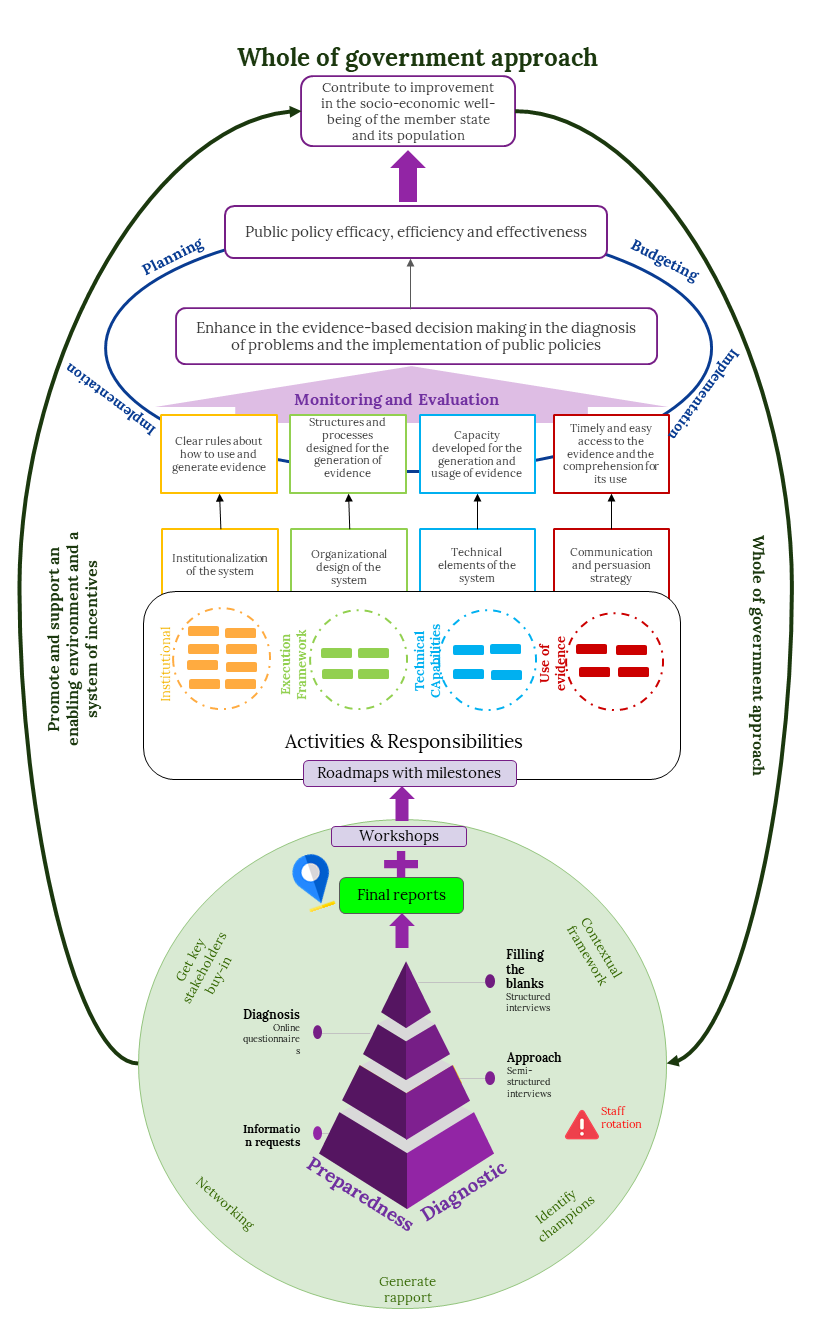
\includegraphics[width=1\linewidth]{./images/figure_1} \caption{Theory of Change}\label{fig:figure1}
\end{figure}

As these four dimensions advance and become solid practices, beyond compliance, the system moves towards an increase in evidence-based decision making across government and across planning, budgeting, and implementation that makes it possible to increase public policies' efficiency, efficacy, and effectiveness.

As the RBM system is sustained and it continues to matures, the dimensions will continue to strengthen, and the enabling environment will promote an RBM culture that ultimately contributes to the improved well-being of all citizens.

\hypertarget{ideal-rbm-system-and-working-process}{%
\section{Ideal RBM system and working process}\label{ideal-rbm-system-and-working-process}}

The development of an RBM System is a complex and nonlinear process that must be contextualized to the specific region, country, or institution. To establish a roadmap to strengthen or build an RBM system, the following three elements are considered:

\begin{enumerate}
\def\labelenumi{\arabic{enumi}.}
\tightlist
\item
  A benchmark against which to assess the level of maturity dubbed as ``Ideal RBM System''
\item
  A methodology to obtain general and specific recommendations and,
\item
  A working process and approach to generate ownership
\end{enumerate}

The Ideal RBM system was established based on the good practices and lessons learned from multiple RBM initiatives in various contexts. These good practices represented useful inputs to determine ideal features of an RBM System. The CLEAR LAC team engaged in this collaboration defined four dimensions of an ideal sustainable RBM system (see \protect\hyperlink{fig:figure2}{Figure 2}):

\begin{figure}
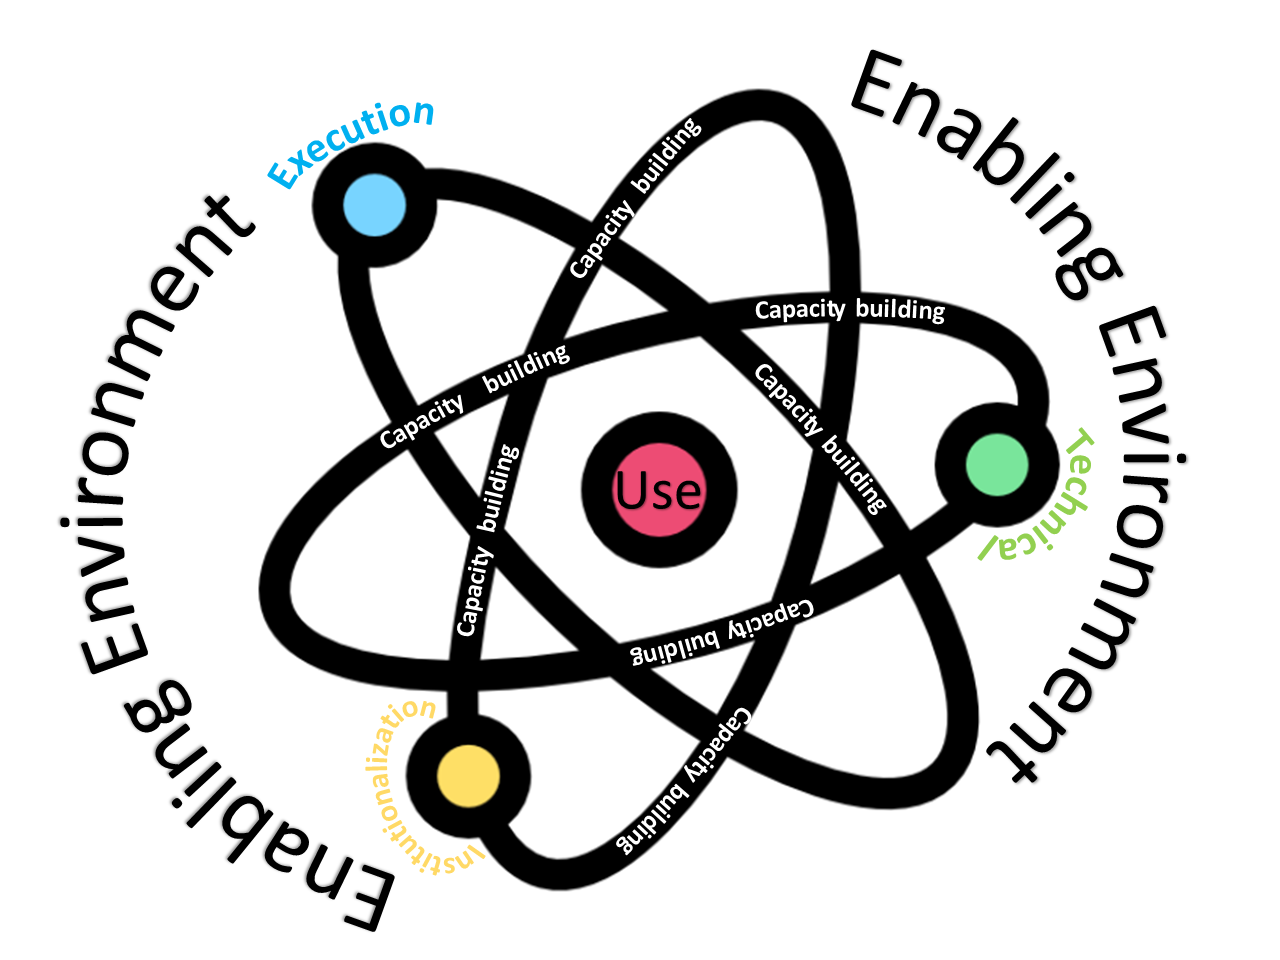
\includegraphics[width=1\linewidth]{./images/figure_2} \caption{Dimensions of an ideal RBM system}\label{fig:figure2}
\end{figure}

\begin{itemize}
\item
  \emph{Institutionalisation:} this dimension focuses on the formal rules that outline the RBM policy in the countries.
\item
  \emph{Execution framework:} this dimension focuses on the systems, resources, processes, methodologies, and tools necessary for the implementation of an RBM system, as well as on the enabling environment.
\item
  \emph{Technical capabilities:} this dimension focuses on the necessary capacities and abilities to implement an RBM System.
\item
  \emph{Use of evidence:} this dimension focuses on the dissemination strategies and incentives aimed at stakeholders with the purpose that they use the evidence generated by the RBM System.
\end{itemize}

Each dimension is integrated by key elements that constitute specific documents, normative frameworks, activities, incentives, among others. These different elements facilitate the operationalisation of the dimension as part of an RBM System. In a third level (beneath dimensions and elements), each element has sub-elements that list their ideal characteristics.

Once all the required information is gathered and analysed (based on the dimension-element-subelement structure), the dimensions will be assessed using a 3-level scale for each sub-element (no, yes, need of improvement)\footnote{For more details on the 3-level scale see \protect\hyperlink{appendixA}{appendix A}} . For this last step, the degree of advance in each sub-element within an element is added up to end up with a value of advance for each element; afterwards, all the element values within each dimension are added up to find the degree of progress of each dimension.

Finally, the average from the progress of the four dimensions places each Member State in a specific level of progress (Early initiatives; Committed development; Growing RBM system; Consolidated practices, or Mature state) in the development and implementation of an RBM System (see \protect\hyperlink{appendixA}{appendix A} for more details).

The working process, defined for this collaboration, identifies Monitoring and Evaluation (M\&E) activities as central elements to be developed and applied to influence planning, budgeting, and implementation. \protect\hyperlink{fig:figure3}{Figure 3} presents the working process and highlights the importance of evidence-based decision making (guided and made feasible by M\&E activities and supported, strengthened, and made sustainable through learning and accountability).

\begin{figure}
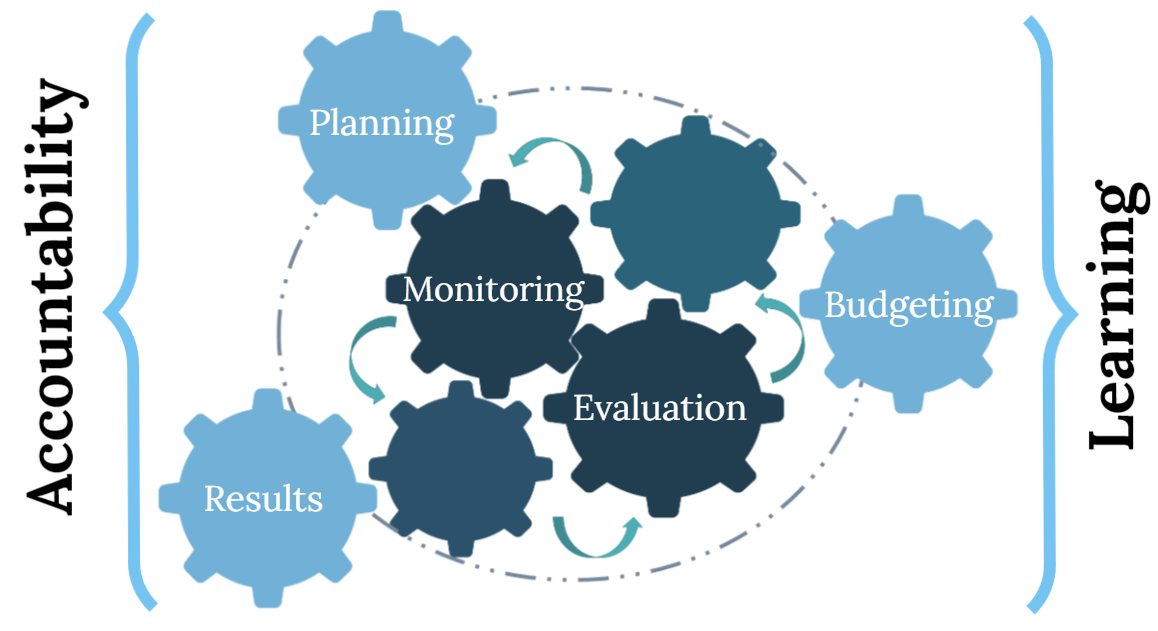
\includegraphics[width=1\linewidth]{./images/figure_3} \caption{Working Process defined for the CARICOM Collaboration}\label{fig:figure3}
\end{figure}

One significant component to strengthen RBM in the Community is to build, through a participatory process, specific roadmaps to continue the development of RBM Systems for each pilot member state and Regional Institution. The Member States and Regional Institutions participating in the pilot have relevant but heterogeneous advances achieving this goal. To identify these advances, guide the analysis of the Preparedness Diagnostic stages, and develop ownership, the roadmap will be developed in workshops with key stakeholders involved in different levels (management, coordination, and operation).

\hypertarget{stages-of-the-preparedness-diagnostic}{%
\section{Stages of the Preparedness Diagnostic}\label{stages-of-the-preparedness-diagnostic}}

The Preparedness Diagnostic (PD) is a four-stage methodology designed to gain a deep understanding of a Member State's relevant aspects/characteristics when developing an RBM System. One main assumption behind the methodological design of the PD is that building a sustainable RBM System requires the active involvement of multiple stakeholders. The stages of the PD use different data collection methods to identify and engage these stakeholders as well as obtaining information to understand the current policy environment; stakeholder's interests, their roles, motivations, relationship dynamics; map existing institutional structures, practices, and mechanisms; and define capacity building needs.

To successfully execute the PD for this collaboration, the CLEAR LAC team, in collaboration with CARICOM Secretariat, selected Executive Coordinators who are representatives for the collaboration from the three Member States (Dominica, Jamaica and Saint Lucia) and the three Regional Institutions (the Caribbean Development Fund, the Caribbean Examinations Council and the CARICOM Implementation Agency for Crime and Security). The role of the Executive Coordinators was key to execute the PD as they have an overall knowledge of their Member State or Regional Institution and have experience in RBM as they have been part of the efforts of their Member State or Regional Institution. As Executive Coordinators for this collaboration, they acted as focal points and contributed to identifying and reaching relevant stakeholders at different stages of the PD and acted as key informants given their experience.

\hypertarget{stages-of-the-pd}{%
\subsection*{Stages of the PD}\label{stages-of-the-pd}}
\addcontentsline{toc}{subsection}{Stages of the PD}

The four stages of the PD (presented in \protect\hyperlink{fig:figure4}{Figure 4} ) are implemented according to a specific sequence and were customized based on the findings of the previous stage. They also involve the participation of different stakeholders to obtain a broad perspective of the pilot Member States and Regional Institutions. The figure below provides a brief description of the approach for implementing the stages.

\begin{figure}
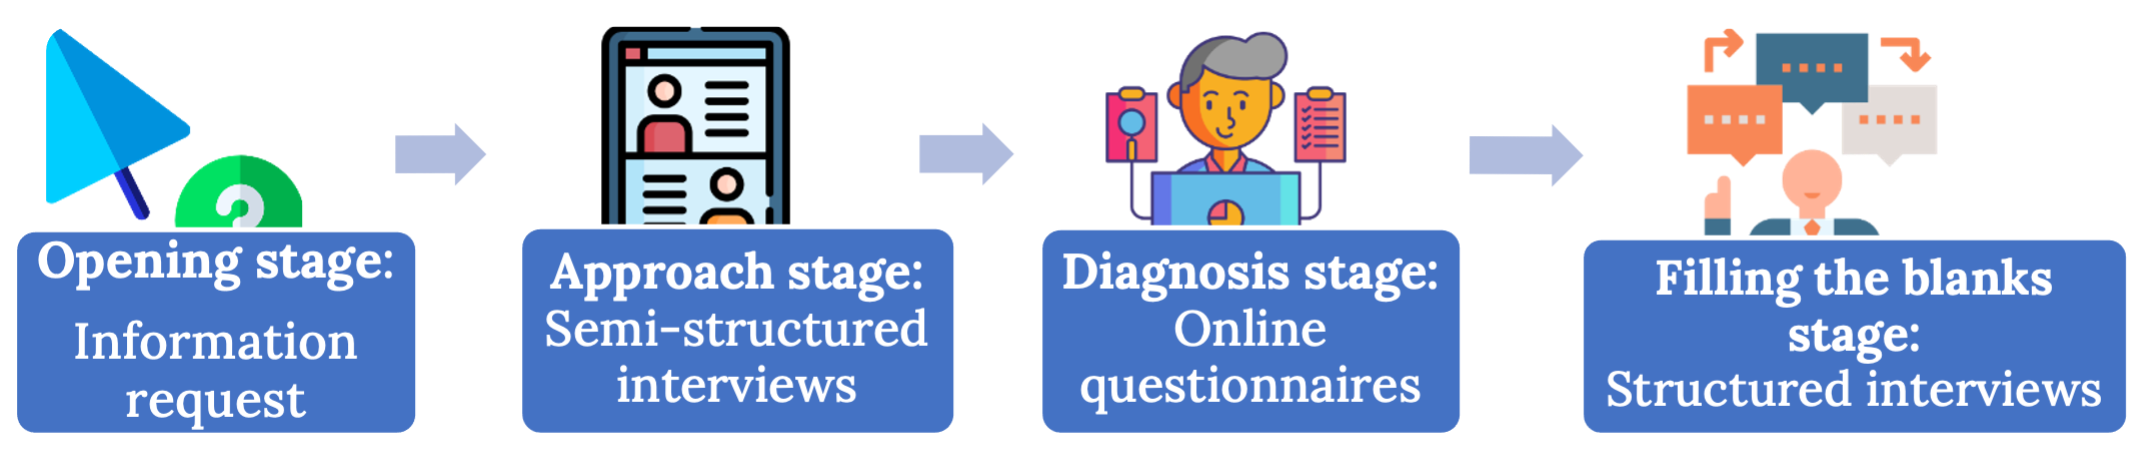
\includegraphics[width=1\linewidth]{./images/figure_4} \caption{Stages of the Preparedness Diagnostic}\label{fig:figure4}
\end{figure}

The \textbf{Opening stage} consisted of a request for different documents from the Executive Coordinators, regarding the pilots' planning, budgeting, and M\&E practices. The desk review and analysis of these documents, in addition to other publicly available information, allowed the design of targeted customized questions for each pilot in the next stage.

The \textbf{Approach stage} involved the identification of various key stakeholders with the support of the Executive Coordinators and the CARICOM Secretariat. The semi-structured interviews addressed general themes that allowed the team to develop rapport with relevant actors within the pilots, as well as obtain additional information about the pilots' current policy environment.

The \textbf{Diagnosis stage} consisted of a series of online questionnaires for the Ministries, Agencies, and Departments of Member States, and Units of Regional Institutions. This stage aimed to gather more in-depth information to complement what was already gathered in previous stages, and to deepen in a whole of government approach. The participants were able to respond to questions and upload documents in a timeframe of approximately four weeks, as well as consult with other stakeholders for any additional information within their pilot Member States or Regional Institution.

Finally, the \textbf{Filling-the-blanks} stage was aimed at addressing information gaps from the previous stages through a series of structured interviews. This stage targeted other stakeholders such as members of Parliament, representatives of multilateral international organizations, development partners, etc.

All the information gathered in the four stages was systematized and analysed to present the findings in this document.

\begin{longtable}[]{@{}
  >{\raggedright\arraybackslash}p{(\columnwidth - 4\tabcolsep) * \real{0.1957}}
  >{\centering\arraybackslash}p{(\columnwidth - 4\tabcolsep) * \real{0.3261}}
  >{\raggedleft\arraybackslash}p{(\columnwidth - 4\tabcolsep) * \real{0.4783}}@{}}
\caption{\label{tab:table1} Dominica's Preparedness Diagnostic Numbers}\tabularnewline
\toprule
\endhead
& \textbf{Stage 1 -- Opening} & Information request to Executive Coordinator + document analysis (+50 documents) + research on official websites. \\
& \textbf{Stage 2 -- Approach} & 7 semi-structured interviews were conducted by the CLEAR LAC team with relevant stakeholders from different MDAs \\
& \textbf{Stage 3 -- Diagnosis} & +100 online questionnaires were sent to MDAs and were answered with both the whole-of-government and MDA approaches. \\

\includegraphics{./images/tb1_4.png} & \textbf{Stage 4 -- Filling the blanks} & No structured interviews were conducted by the CLEAR LAC team. \\
& & \\
\bottomrule
\end{longtable}

\hypertarget{strengths-of-the-pd}{%
\subsection*{Strengths of the PD}\label{strengths-of-the-pd}}
\addcontentsline{toc}{subsection}{Strengths of the PD}

\begin{itemize}
\item
  Different stages were designed to identify specific stakeholders and to generate rapport with them.
\item
  As the stages are implemented and analysed sequentially, different layers of information are gathered
\item
  Participatory process that leads to the Member States or RI's ownership of the collaboration
\item
  Qualitative and quantitative mixed methods used
\end{itemize}

All stages are adapted for to consider the context of each Member State or RI

\hypertarget{limitations-of-the-pd}{%
\subsection*{Limitations of the PD}\label{limitations-of-the-pd}}
\addcontentsline{toc}{subsection}{Limitations of the PD}

\begin{itemize}
\item
  Specific results for one pilot cannot be generalized to others given the customization of the instruments and contextual differences among them
\item
  There are time limitations due to tight agendas of stakeholders that complicates reaching all the desired informants.
\item
  All stages were implemented remotely, and it is preferred to have some face-to-face contact with the stakeholders in at least one of the stages to generate rapport
\item
  The duration of the PD is approximately six effective months; however this was extended due to the whole of government/institution approach and the stakeholders' agendas.
\end{itemize}

\hypertarget{section4}{%
\chapter[Dominica's profile]{\texorpdfstring{Dominica's profile\footnote{Centro de Estudios Internacionales Gilberto Bosques. (april, 2020). Mancomunidad de Dominica. Ficha Técnica. \url{https://centrogilbertobosques.senado.gob.mx/docs/F_Dominica.pdf}}}{Dominica's profile}}\label{section4}}

Dominica, officially Commonwealth of Dominica, is an island country in the Caribbean, and is part of the Lesser Antilles archipelago. The country has a population of 72,344 people and around 16,571 of its habitants are concentrated in the capital city of Roseau\footnote{World Population Review. Dominica Population 2022. \url{https://worldpopulationreview.com/countries/dominica-population}} . Dominica became a member of the West Indian Federation in 1958 in its search for independence and was granted independence as a republic in 1978, after becoming an associate state of the United Kingdom in 1967.

Dominica is a parliamentary democracy. As a Republic, the head of State is the president, who is elected for a five-year term by the parliament after being nominated by the prime minister and the opposition leader. The executive branch also includes the prime minister, the head of the government, who is the leader of the majority party in the parliament and is appointed by the president.

The Legislative branch is made up of the House of Representatives, with a total of 32 members; 21 are regional representatives elected for a five-year term and 9 are senators appointed by the president, five on the advice of the prime minister, and four on the advice of the opposition leader. The president is also considered a member of the parliament, and the last seat is for the speaker of the House of Assembly, elected by the elected members after an election. The latest general elections were held on December 2019 resulting in a victory for the ruling party, the Dominica Labour Party.

As a small country, Dominica mainly relies on its membership in international and regional organizations to make its vote count, therefore most of its foreign policy is exercised through these forums. At the international level, Dominica is a member of CARIFORUM, CARICOM, the Organization of Eastern Caribbean States, and the Organization of American States (OAS).

\begin{longtable}[]{@{}
  >{\raggedright\arraybackslash}p{(\columnwidth - 4\tabcolsep) * \real{0.1935}}
  >{\centering\arraybackslash}p{(\columnwidth - 4\tabcolsep) * \real{0.4839}}
  >{\raggedleft\arraybackslash}p{(\columnwidth - 4\tabcolsep) * \real{0.3226}}@{}}
\caption{\label{tab:table2} General Statistics of Dominica}\tabularnewline
\toprule
\endhead
& \textbf{Gross Domestic Product\footnote{Consulted in: \url{https://data.worldbank.org/indicator/NY.GDP.MKTP.CD?locations=DM}}} & 504.2M USD (nominal, 2020) Position 188/216 \\
& \textbf{Main economic activities\footnote{Consulted in: \url{https://www.cia.gov/the-world-factbook/countries/dominica/\#economy}}} & Services (65.1\%) Agriculture ( 22.3 \% ) Industry (12.6\%) \\
& \textbf{Inflation rate\footnote{Consulted in: \url{https://data.worldbank.org/indicator/FP.CPI.TOTL.ZG?locations=DM}}} & -0.73 (2020) \\
& \textbf{Population\footnote{Consulted in: \url{https://data.worldbank.org/indicator/SP.POP.TOTL?locations=DM}}} & 71,991 (2020) \\
& \textbf{Poverty\footnote{Consulted in: \url{https://www.cia.gov/the-world-factbook/countries/dominica/\#economy}}} & 29\% (2009 below international poverty line) \\
& & \\
\bottomrule
\end{longtable}

\hypertarget{dominicas-rbm-profile}{%
\section{Dominica's RBM profile}\label{dominicas-rbm-profile}}

The government of Dominica has set a clear long-term goal to be achieved: to become the first climate-resilient country in the world. After the passage of a Category 5 Hurricane in 2017, the nation was challenged to recover from damages and losses estimated at 226\% of its GDP. It was acknowledged that an integrated national RBM System must be implemented to achieve this ambitious goal.

There have been significant efforts in terms of planning to translate Dominica's bold vision into a reality, using a results-oriented approach. The creation of the Climate Resilient Executive Agency for Dominica (CREAD), an agency with different mandates and functions to transform Dominica's vision into a reality constitutes a significant step to ensure that government interventions stay on track and the intended results are delivered. The National Resilient Development Strategy 2030 (NRDS) provides a path with specific results to be achieved by 2030, all within a framework oriented to becoming a climate-resilient country. This plan was complemented with Dominica's Climate Resilience and Recovery Plan 2020--2030 (CRRP), a document that operationalises the NRDS and has a robust monitoring matrix that facilitates the tracking of priority initiatives, as well as identifying responsibilities for its implementation.

In terms of M\&E, there are significant advances in the implementation of coordinated monitoring activities. The Ministry of Planning, Economic Development, Climate Resilience, Sustainable Development, and Renewable Energy (Ministry of Planning from here on) coordinates periodic monitoring exercises with all the ministries. On a monthly basis, the ministries submit a report (with programmatic and financial data) to the Ministry of Planning to track the progress made in implementing the planned activities, assess the achievement of outputs and outcomes, as well as the budget implementation by the source of funds. Also, the government is working on the development of a Monitoring and Evaluation Framework as part of a national effort to introduce an integrated results-based management system within the public sector.

Regarding the national budget, there are different normative frameworks that guide the budgeting activities in Dominica. Both the Ministries of Planning and the Ministry of Finance and Investment (Ministry of Finance from here on) oversee the development of the national budget. The Ministry of Finance has the overall responsibility for the preparation of the budget. In the case of the interventions included in the Public Sector Investment Programme (PSIP), information on its past performance is requested in the Budget Application.

Multiple stakeholders have acknowledged the importance of developing and implementing a sustainable RBM System in Dominica. Having the aspirational vision of becoming the first climate-resilient country in the world requires the adoption of a results-oriented approach that is transversal in the planning, budgeting, and implementation activities performed by the government. It is crucial to ensure that the public sector is focused on achieving the targets set in the national planning, and systematic M\&E activities will allow them to track their efforts and stay on track.

\hypertarget{section5}{%
\chapter{Main findings}\label{section5}}

As mentioned above, this Preparedness Diagnostic uses four dimensions analysis as a reference. Each dimension contains elements considered relevant to have an ``Ideal RBM System''. This Ideal RBM System will allow us to compare the current situation in Dominica in relation to the best possible scenario regarding RBM, its practices, uses and results. Figure 5 shows the progress rate of each of the dimensions analysed, with respect to the ideal scenario.

The elements and sub-elements of the reference Ideal RBM System are not a ``natural'' condition. This means that each one must be designed and developed; following this, a country that has not considered adopting RBM practices would probably not comply or show advances in any of the analysed elements. In this sense, all the advances identified in this diagnosis represent valuable progress.

It is important to mention that, although there is a numerical value for each dimension, behind the numbers there was a qualitative analysis that determined the current situation of Dominica regarding RBM. Furthermore, these ``ratings'' are in terms of the ideal scenario, so in no way does it represent an outright success or failure, but rather a proxy to the best possible situation of the RBM.

\begin{longtable}[]{@{}
  >{\raggedright\arraybackslash}p{(\columnwidth - 2\tabcolsep) * \real{0.3889}}
  >{\raggedright\arraybackslash}p{(\columnwidth - 2\tabcolsep) * \real{0.3472}}@{}}
\caption{\label{tab:table} Developed by the CLEAR LAC technical team in charge of the collaboration}\tabularnewline
\toprule
\begin{minipage}[b]{\linewidth}\raggedright
DIMENSION
\end{minipage} & \begin{minipage}[b]{\linewidth}\raggedright
LEVEL OF PROGRESS
\end{minipage} \\
\midrule
\endfirsthead
\toprule
\begin{minipage}[b]{\linewidth}\raggedright
DIMENSION
\end{minipage} & \begin{minipage}[b]{\linewidth}\raggedright
LEVEL OF PROGRESS
\end{minipage} \\
\midrule
\endhead
INSTITUTIONALISATION & 22\% \\
EXECUTION FRAMEWORK & 9\% \\
TECHNICAL CAPABILITIES & 28\% \\
USE OF EVIDENCE & 14\% \\
\bottomrule
\end{longtable}

\begin{figure}

{\centering 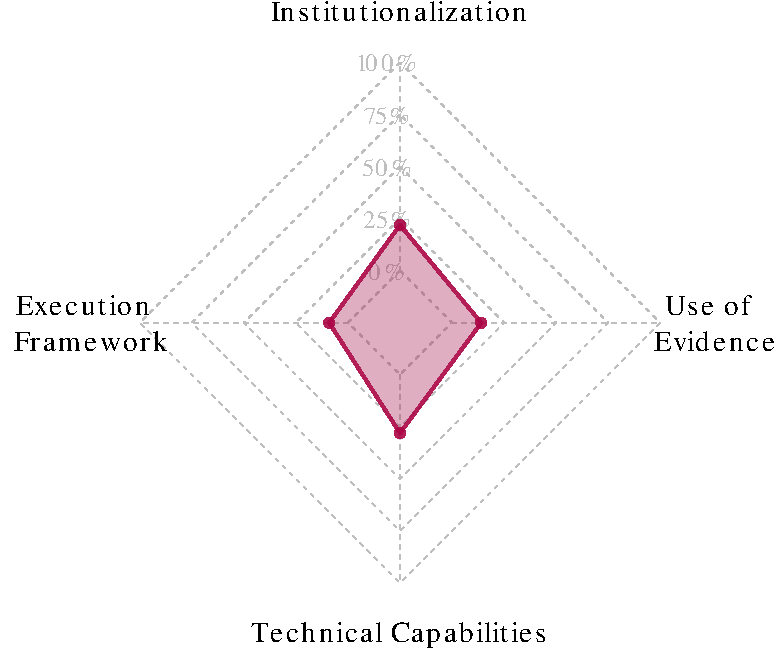
\includegraphics[width=0.7\linewidth]{09-section5_files/figure-latex/figure5-1} 

}

\caption{Level of progress of the Ideal RBM System}\label{fig:figure5}
\end{figure}

Considering this level of progress, a metric was built to progressively identify five levels of maturity of RBM systems. In this way, the progress levels presented above are averaged to characterise the Member State's level . The 5 levels are:

\begin{enumerate}
\def\labelenumi{\arabic{enumi}.}
\tightlist
\item
  Early initiatives
\item
  Committed development
\item
  Growing RBM System
\item
  Consolidated practices
\item
  Mature State
\end{enumerate}

Based on the results from the Preparedness Diagnostic analysis, Dominica is currently in the Early initiatives level. Significant efforts have been made in developing and implementing a results-oriented national planning with clear strategies that contribute to the achievement of Dominica's higher goal of climate resiliency. There are also initial efforts in monitoring activities; however, they are not articulated and there are no clear responsible stakeholders in the monitoring process. It is pending for Dominica to start the drafting of an RBM Policy and the building of a whole-of-government, to develop evaluation activities, to define an incentives structure to build an enabling environment that ensures the sustainability of an RBM System.

\hypertarget{results-by-dimension}{%
\section{Results by dimension}\label{results-by-dimension}}

The results of this diagnosis for each of the dimensions analysed (and their ideal elements) are presented below in a synthetic manner. For more detailed information on each dimension, elements, and sub-elements, please see \protect\hyperlink{appendixC}{appendix C} and visit the interactive platform with all the disaggregated findings of this PD.

\hypertarget{institutionalisation}{%
\subsection{Institutionalisation}\label{institutionalisation}}

\begin{longtable}[]{@{}
  >{\raggedright\arraybackslash}p{(\columnwidth - 2\tabcolsep) * \real{0.6136}}
  >{\raggedright\arraybackslash}p{(\columnwidth - 2\tabcolsep) * \real{0.3864}}@{}}
\toprule
\begin{minipage}[b]{\linewidth}\raggedright
Key Message
\end{minipage} & \begin{minipage}[b]{\linewidth}\raggedright
\end{minipage} \\
\midrule
\endhead
Dominica has broad normative frameworks in planning, significant advances in budgeting, and slight advances in monitoring. The Climate Resilience Executive Agency for Dominica (CREAD), a cross-cutting and temporary institution created to achieve Dominica's long-term goal (become the first climate resilient nation), plays a relevant role in supporting MDAs in the monitoring and implementation of programmes. However, there are not enough norms and clear responsibilities to foster the continuous improvement in planning, budgeting, and implementation based on the use of M\&E results, and to articulate a whole of government RBM system. & \\
\textbackslash includegraphics{[}width=120\%{]}\{./images/dim\_1\} & \\
& \\
\bottomrule
\end{longtable}

\begin{longtable}[]{@{}
  >{\raggedright\arraybackslash}p{(\columnwidth - 2\tabcolsep) * \real{0.5972}}
  >{\raggedright\arraybackslash}p{(\columnwidth - 2\tabcolsep) * \real{0.3472}}@{}}
\toprule
\begin{minipage}[b]{\linewidth}\raggedright
Ideal element \textbar{}
\end{minipage} & \begin{minipage}[b]{\linewidth}\raggedright
LEVEL OF PROGRESS
\end{minipage} \\
\midrule
\endhead
\begin{minipage}[t]{\linewidth}\raggedright
\begin{enumerate}
\def\labelenumi{\arabic{enumi}.}
\tightlist
\item
  There is a documented, approved, and bin
\end{enumerate}
\end{minipage} & ding RBM Policy within the government \textbar{} 22\% \\
\bottomrule
\end{longtable}

\hypertarget{main-challenges-to-strengthen-the-rbm-system}{%
\section{Main challenges to strengthen the RBM system}\label{main-challenges-to-strengthen-the-rbm-system}}

As mentioned in section 2.2, the development of an RBM System is a complex, nonlinear, and continuous process that must be contextualized in each country. In doing so, it is important to consider the main challenges that Dominica faces when it comes to strengthening its RBM system. This diagnosis identifies three major challenges:

\begin{enumerate}
\def\labelenumi{\arabic{enumi}.}
\item
  Changing the culture and fostering the enabling environment to have an RBM system in place implies a change of mindset of public servants at all levels. It should be considered that throughout the process there must be a constant awareness/sensitization strategy, both in the short and medium term, that allows public servants to identify the importance to have this mindset change in pursuit of RBM. In other words, on a regular basis, there needs to be reminders on the importance of RBM and its impact on improving performance and lives of all citizens
\item
  Since this collaboration constitutes a whole-of-government approach, it is necessary to have a top-bottom commitment in which leaders and decision-makers demonstrate the benefits of the RBM system through evidence informed actions that are generated by the RBM system. This means that we need a top-bottom approach to use, and thereby demonstrate its usefulness, the information and evidence derived from the RBM system to improve planning and budgeting decisions.
\item
  For the RBM system to be sustainable, it is critical to generate a system of incentives and ensure that there is a balance between positive and negative incentives (such as potential penalties for non-compliance), to advance and sustain the system. The positive incentives can take different forms, from monetary to symbolic, such as the presentation of awards to staff and units and recognition for good performance in public service.
\end{enumerate}

\hypertarget{section6}{%
\chapter{Next steps to building the roadmap}\label{section6}}

RBM entails more than just abiding with certain requirements. Compliance is in adequate since it entails a change of mindset on the way things are done. This change of mindset involves different areas and stages of a government period. Having reviewed the main results from the preparedness diagnostic in terms of the dimensions of elements considered as part of an ideal RBM system, this section introduces the next steps that will be carried out as part of the process of building contextualized roadmaps.

The roadmap will present pathways to influence planning, budgeting, implementation, and the M\&E functions, as well as the promotion of accountability and learning. The main objective is for Dominica to have a defined action course that also specifies responsibilities and shows the importance of the participation of all relevant stakeholders.

\begin{figure}
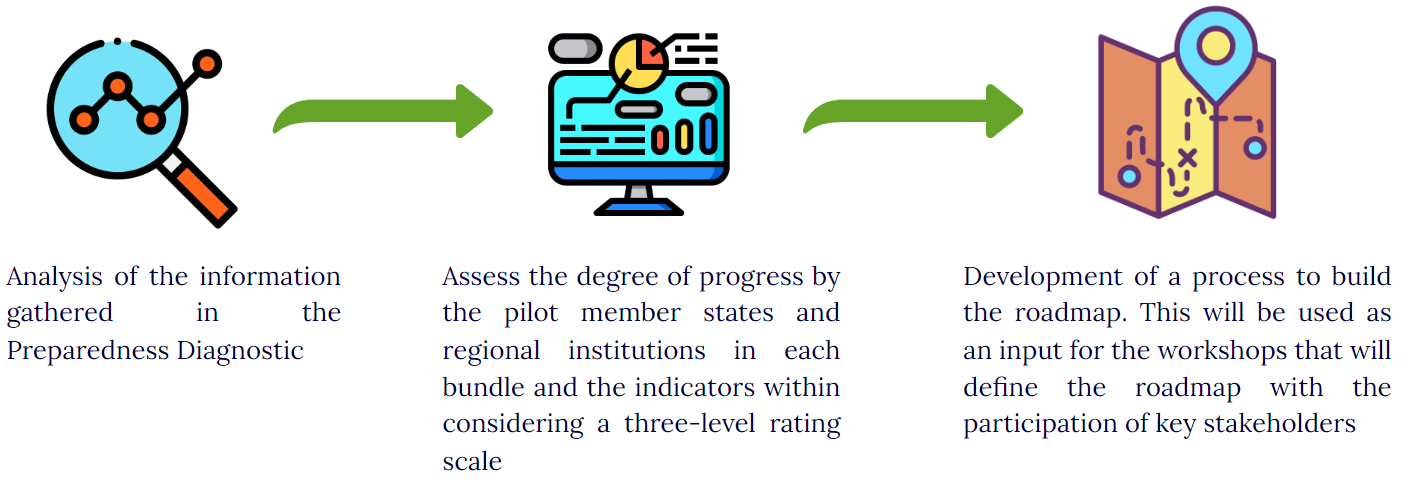
\includegraphics[width=1\linewidth]{./images/figure_6} \caption{From an ideal RBM system to the roadmaps}\label{fig:figure6}
\end{figure}

The whole process has a coproduction approach, were aside of the CLEAR LAC team, the CARICOM Secretariat, and the Executive Coordinators, key stakeholders will be involved in a fluid process to develop a learning loop for feedback and process improvement.

\begin{figure}
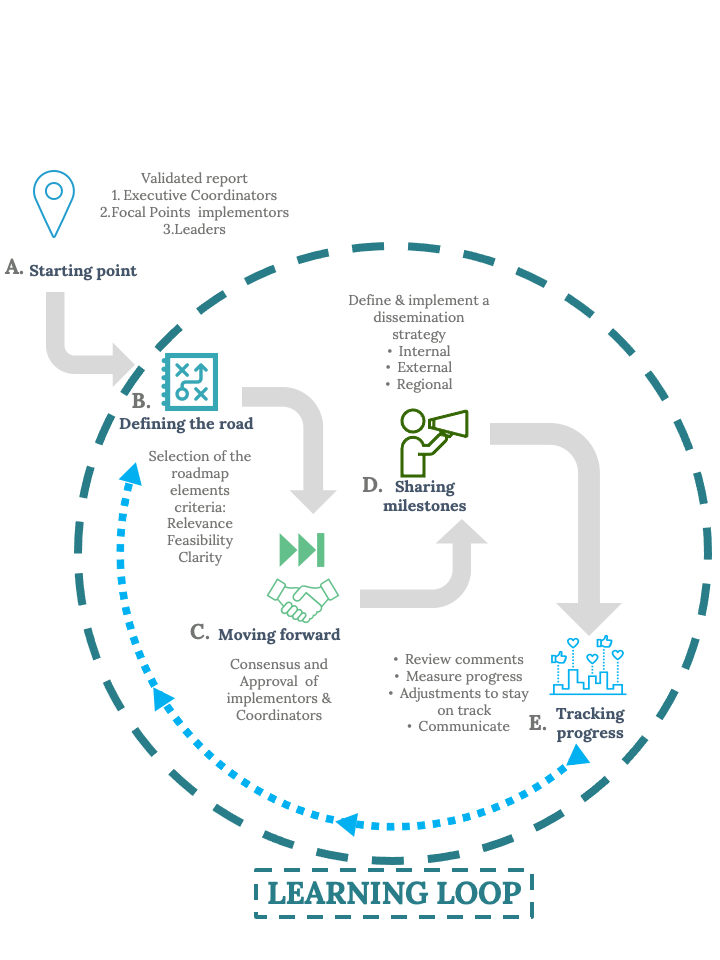
\includegraphics[width=1\linewidth]{./images/figure_7} \caption{Learning loop}\label{fig:figure7}
\end{figure}

This report is considered as the \emph{starting point} in this process; take into consideration that, as \protect\hyperlink{fig:figure7}{figure 7} illustrates, the process started before its publication.

Once the first draft was completed, it will be shared with key stakeholders for review and validation, starting with the Executive Coordinators. Once the feedback period concluded, the report itself became an input for what is to come and will be disseminated to generate knowledge, support the sensitisation and empowerment of key stakeholders to strengthen RBM practices, and promote ownership of the next steps.

The next steps start with \emph{defining the road}, engaging key stakeholders to coproduce contextualized medium term roadmaps that will include specific activities and milestones that will facilitate implementation. To develop the roadmap, the CLEAR LAC team has designed a series of workshops with the participation of stakeholders involved in the different areas and levels of what is to be the national RBM system, and that have been carefully identified as part of the PD process.

To \emph{move forward}, this first draft of the roadmap is presented to other relevant stakeholders to build consensus and support for the process. It is crucial to gain whole-of-government ownership, so it is important to define and implement a dissemination strategy for \emph{sharing milestones} in different levels: internal, external and regional, once they have been clearly defined and responsibilities have been assigned. Finally, it is important to \emph{track the progress} of implementation and communicate results to ensure that the Member State learns from the process, adjusts and stays in the correct path. The continuum process of identifying, sharing, reviewing, and adjusting represents a learning loop.

\hypertarget{stakeholders-contribution-analysis}{%
\section{Stakeholders' contribution analysis}\label{stakeholders-contribution-analysis}}

This section presents an analysis of stakeholders to identify which of them are relevant to strengthening the RBM system. Each of these stakeholders are involved in the decision making and execution at varied levels. Based on the CLEAR LAC's team analysis, a proposal of the possible contribution of the stakeholders (considering positions and experience) is summarised below to support the improvement of the system which will generate the necessary evidence and results for decision-making planning, budgeting .

The analysis is summarized (but not limited only, due to the constant change in the dynamics in which the stakeholders relate) in the following table. During the roadmap development workshops that will be held with government stakeholders, new stakeholders could be identified or some of those presented here could be discarded. Once its RBM Policy is approved and published, we will be able to have greater clarity on the roles, responsibilities, capacities, and relevance of the stakeholders that will integrate the system both at MDA and whole-of-government approach.

\hypertarget{references-sources}{%
\chapter*{References \& Sources}\label{references-sources}}
\addcontentsline{toc}{chapter}{References \& Sources}

\begin{itemize}
\item
  Centro de Estudios Internacionales Gilberto Bosques. (april, 2020). Mancomunidad de Dominica. Ficha Técnica. \url{https://centrogilbertobosques.senado.gob.mx/docs/F_Dominica.pdf}
\item
  Dominica Population 2022 (Demographics, Maps, Graphs). (2022). World Population Review. \url{https://worldpopulationreview.com/countries/dominica-population}
\item
  Editors of Encyclopedia Britannica. (s. f.). Dominica summary. Encyclopedia Britannica. \url{https://www.britannica.com/summary/Dominica}
\item
  Freedom House. (2020). Dominica. \url{https://freedomhouse.org/country/dominica/freedom-world/2020}
  World Population Review. Dominica Population 2022. \url{https://worldpopulationreview.com/countries/dominica-population}
\end{itemize}

\hypertarget{appendix-appendix}{%
\appendix}


\hypertarget{appendixA}{%
\chapter{Conceptual framework (CLEAR LAC)}\label{appendixA}}

\hypertarget{key-dimensions-of-a-sustainable-rbm-system}{%
\section{Key dimensions of a sustainable RBM System}\label{key-dimensions-of-a-sustainable-rbm-system}}

The development of an RBM System is a complex and nonlinear process that must be contextualized to the specific region, country, or Regional Institution. However, the multiple efforts done over time allow us to learn from experiences in different settings and identify good practices. These good practices represent useful inputs to be considered when embarked on this road.

One significant component to strengthen RBM in the Community is to build, in a participatory process, specific roadmaps to continue the development of RBM Systems for each pilot member state and Regional Institution. The Member States and Regional Institutions participating in the pilot have significant but heterogeneous advances achieving this goal. To identify these advances and guide the analysis of the Preparedness Diagnostic stages, the CLEAR LAC team defined four dimensions of an ideal and sustainable RBM System:

\begin{itemize}
\item
  \emph{Institutionalisation:} this dimension focuses on the formal rules that defines, outlines and formalize the RBM Systems in the countries.
\item
  \emph{Execution framework:} this dimension focuses on the systems, resources, processes, methodologies, and tools necessary for the implementation of the RBM system, as well as incentives that promote an enabling environment.
\item
  \emph{Technical capabilities:} this dimension focuses on the capacities, abilities, and resources necessary to implement and sustain the RBM System.
\item
  \emph{Use of evidence:} this dimension focuses on the dissemination strategies and incentives aimed at stakeholders with the purpose that they use the evidence generated by the RBM System and its measurement.
\end{itemize}

\hypertarget{ideal-elements-sub-elements}{%
\section{Ideal elements \& sub-elements}\label{ideal-elements-sub-elements}}

The four dimensions previously mentioned were conceptualized as necessary components when building an operating and sustainable RBM system. To have a better understanding of what the progress in each dimension entails, we propose a set of ideal elements and sub-elements taken from different contexts and experiences where they have been successfully implemented or recommended. Each dimension has a set of elements that represent activities, documents, normative frameworks, skills, incentives, etc.; and every element has a set of sub-elements that describe the ideal characteristics of the element. The sub-elements allow to translate concepts into practice, and, after gathering and analysing information, this knowledge can be translated into specific actions.

Unlike the dimensions, as RBM Systems are designed and built considering contextual factors, some elements and sub-elements should be taken as a guide as different contexts will result in variations on their interpretation and level of relevance/priorities. This framework allows for adaptations, recognizing that every context is particular and that there is no unique checklist that may apply to all contexts.

\hypertarget{levels-of-progress}{%
\section{Levels of progress}\label{levels-of-progress}}

The Preparedness Diagnostic methodology is designed to gain a deep understanding of a country or institution's relevant aspects/characteristics when developing an RBM System. The different stages are meant gather information from different stakeholders to achieve a whole of government / institutional outlook. The dimensions with ideal elements and sub-elements guide the analysis of the information gathered in order to identify the level of progress of a specific government or institution.

The scale used to assess the sub-elements are:
- No: there is no documented advance in the sub-element
- Needs improvement: there is documented advance in the sub-element, but do not cover all the criteria express in the sub-element.
- Yes: there is documented proof that the sub-element complies with the needed/ideal characteristics

Each scale level has an assigned value, and every element will have a result obtained from the total sum of its sub-element's scores. The average score of the elements per dimension results in the dimension's score, and the average score of the four dimensions will place the Member state in one of the following levels of progress of their RBM Systems:

\begin{itemize}
\tightlist
\item
  Level 0. No RBM
\item
  Level 1. Early initiatives: there are some initiatives to develop RBM-related structures and focus on monitoring activities
\item
  Level 2. Committed development: there are RBM-related structures being stablished and limited evaluation activities
\item
  Level 3. Growing RBM System: there are integrated efforts (political will, capacity building and some whole-of-government consensus) to develop the RBM System
\item
  Level 4. Consolidated Practices: M\&E practices are developed continuously and in a structured manner and linked to RBM through budgeting and planning
\item
  Level 5. Mature state: Functioning and sustainable RBM System in place that generates credible, reliable, and timely information that improves public policies
\end{itemize}

\begin{figure}
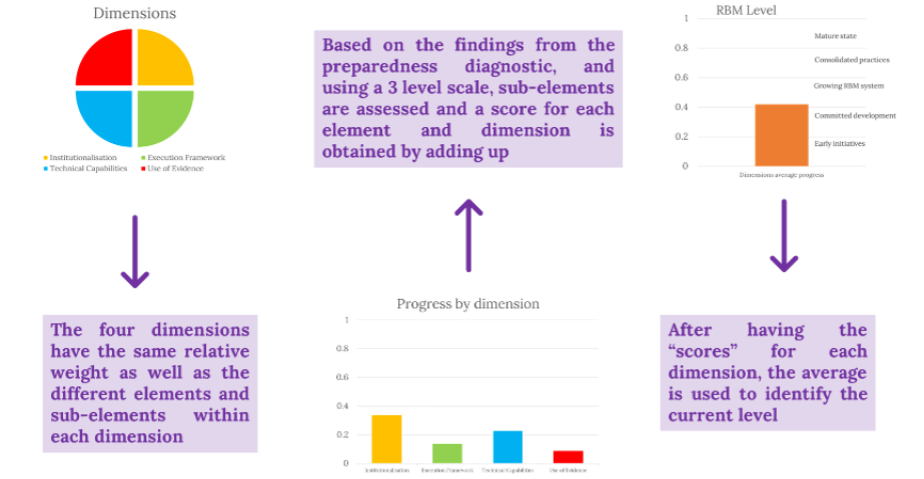
\includegraphics[width=1\linewidth]{./images/figure_8} \caption{How to identify the current level of the RBM system maturity}\label{fig:figure8}
\end{figure}

\hypertarget{appendixB}{%
\chapter{Detailed findings}\label{appendixB}}

In the following table, you can consult all the findings found in this PD in detail. Also, by clicking here (working on the dynamic report) you will be able to consult the detailed findings in an interactive way, navigating through each one of the dimensions, its elements and sub-elements in a simple and clear way.

\hypertarget{appendixC}{%
\chapter{Dominica's budgeting process}\label{appendixC}}

\begin{itemize}
\item
  Every year, there is a budget calendar which is a list of sequence activities conducted by different stakeholders. A budget call is made, and a circular of guidelines to elaborate the budget proposal is sent to the MDAs.
\item
  After that, the MDAs have six weeks to elaborate the proposal. All MDAs submit estimates of recurrent and capital expenditure ; defend budgetary proposals during budget discussions and subsequent bilaterals.
\item
  The Ministry of Planning PSIP Unit reviews capital proposals with estimates; Undertake all tasks associated with the formulation and rationalization of the capital estimates prior to Cabinet approval; Submit capital estimates for Cabinet Approval; Prepare capital templates for Printery.
\item
  The Ministry of Finance reviews and rationalize recurrent proposals; Submit for the approval of Minister of Finance; Prepare and submit recurrent templates to Printery
\item
  The Ministry of Finance sends the budget for final approval to the House of Parliament.
\end{itemize}

\hypertarget{appendixD}{%
\chapter{List of participants in the Preparedness Diagnostic}\label{appendixD}}

\hypertarget{appendixE}{%
\chapter{List of shared documents}\label{appendixE}}

Different stakeholders shared some documents for the Preparedness Diagnostic. The list of documents is the following:

\begin{itemize}
\item
  \textbf{Budget calendar}
\item
  \textbf{Compendium of Strategic priorities by MDA}
\item
  \textbf{CREAD's Policy Paper 1. Strategic Results Planning Framework}
\item
  \textbf{CREAD's Policy Paper 2. Restructuring of the PSIP Process}
\item
  \textbf{CREAD's Policy Paper 3. Improving the Monitoring of PSIP Projects}
\item
  \textbf{CREAD's Policy Paper 4. Improving Performance Through e-Learning}
\item
  \textbf{Dominica Climate Resilience and Recovery Plan 2020 -- 2030}
\item
  \textbf{Finance Administration Act - Act 4 of 1994}
\item
  \textbf{Monthly report template for MDAs}
\item
  \textbf{National Resilience Development Strategy 2030}
\item
  \textbf{National education contacts}
\item
  \textbf{Organizational chart of the Government of Dominica}
\item
  \textbf{Policy and Legislative Framework Matrix to Inform CRRP Implementation Plan}
\item
  \textbf{PSIP budget application}
\end{itemize}

  \bibliography{book.bib,packages.bib}

\end{document}
